\chapter{Results and Analysis}

The results of the project demonstrate the locomotion of quadrupedal robot, which are pitching, yawing, rolling, and squatting. By adjusting parameters through corresponding custom sliders, series of actions are obtained through screenshots and merged into figures, where certain text interpretation would be executed. However, the analysis part will not classify by different actions because the design of programs are similar. On this occasion, integrating common problems for error analysis will be more helpful to the optimization of the program.


\section{Pitching}

Pitching, for the quadruped robot, is the action of rotating about the transverse axis ~\cite{ref:sixDOF}. By pulling the custom slider of pitching to adjust the parameters, a series of actions of the quadruped robot when pitching are shown in Fig.~\ref{fig:pitching}.

\begin{figure}[htbp]
    \centering
    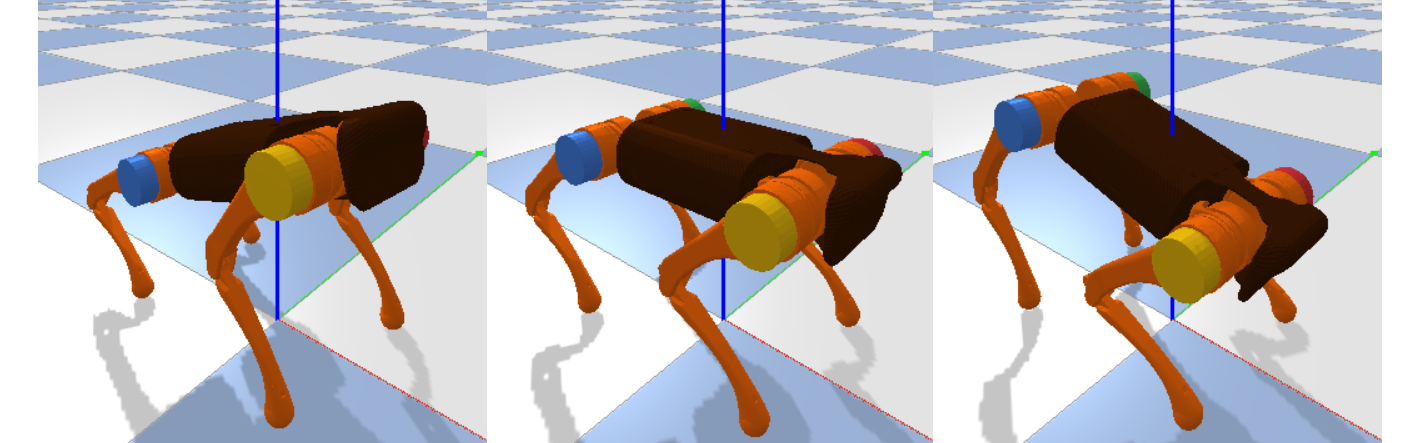
\includegraphics[width=0.8\textwidth]{figures/pitching.png}
    \caption{The result of pitching}
    \label{fig:pitching}
\end{figure}

In the initial position, the body of quadruped robot remained horizontal, which means that the pitch angle was 0. While the slider of debug parameter was pulled to the left, the pitch angle became negative, the body of robot made counterclockwise rotation about transverse axis. While the slider of debug parameter was pulled to the right, the pitch angle became positive, the body of robot made clockwise rotation about transverse axis.


\section{Yawing}

Yawing, for the quadruped robot, is the action of rotating about the normal axis ~\cite{ref:sixDOF}. By pulling the custom slider of squatting to adjust the parameters, a series of actions of the quadruped robot when yawing are shown in Fig.~\ref{fig:yawing}.

\begin{figure}[htbp]
    \centering
    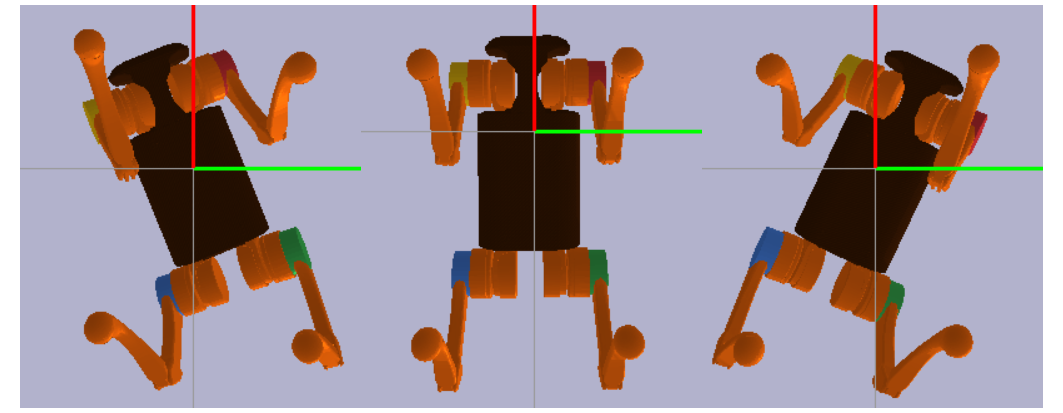
\includegraphics[width=0.8\textwidth]{figures/yawing.png}
    \caption{The result of yawing}
    \label{fig:yawing}
\end{figure}


In order to observe the locomotion of quadruped robot more intuitively, we chose the bottom view as the observation view in the screenshots of yawing. In the initial position, the body of the quadruped robot was parallel to the longitudinal axis, which means that the yaw angle was 0. While the slider of debug parameter was pulled to the left, the yaw angle became negative, the body of robot made counterclockwise rotation about normal axis. While the slider of debug parameter was pulled to the right, the yaw angle became positive, the body of robot made clockwise rotation about normal axis.


\section{Rolling}

Rolling, for the quadruped robot, is the action of rotating about the longitudinal axis \cite{ref:sixDOF}. By pulling the custom slider of squatting to adjust the parameters, a series of actions of the quadruped robot when rolling are shown in Fig. \ref{fig:rolling}.

\begin{figure}[htbp]
    \centering
    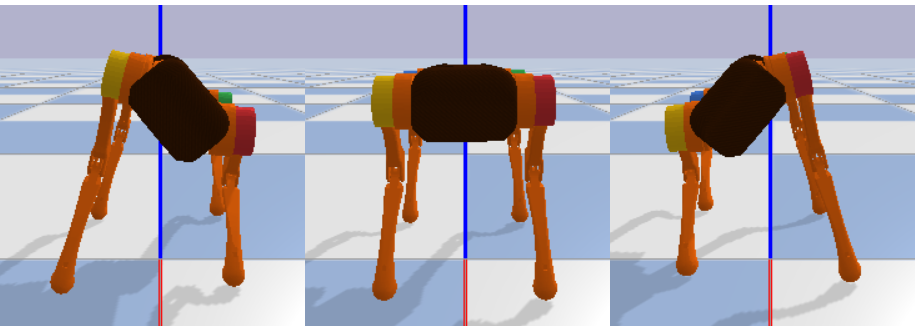
\includegraphics[width=0.8\textwidth]{figures/rolling.png}
    \caption{The result of rolling}
    \label{fig:rolling}
\end{figure}

In order to observe the locomotion of quadruped robot more intuitively, we chose the front view as the observation view in the screenshots of rolling. In the initial position, the heights of the left and right hip joints from the ground are the same, which means that the roll angle was 0. While the slider of debug parameter was pulled to the left, the roll angle became negative, the body of robot made clockwise rotation about longitudinal axis. While the slider of debug parameter was pulled to the right, the roll angle became positive, the body of robot made counterclockwise rotation about longitudinal axis.



\section{Squatting}

Squatting, for the quadruped robot, is the action that make the gravity center of its main body rise or fall vertically. By pulling the custom slider of squatting to adjust the parameters, a series of actions of the quadruped robot when squatting are shown in Fig.~\ref{fig:squatting}.

\begin{figure}[htbp]
    \centering
    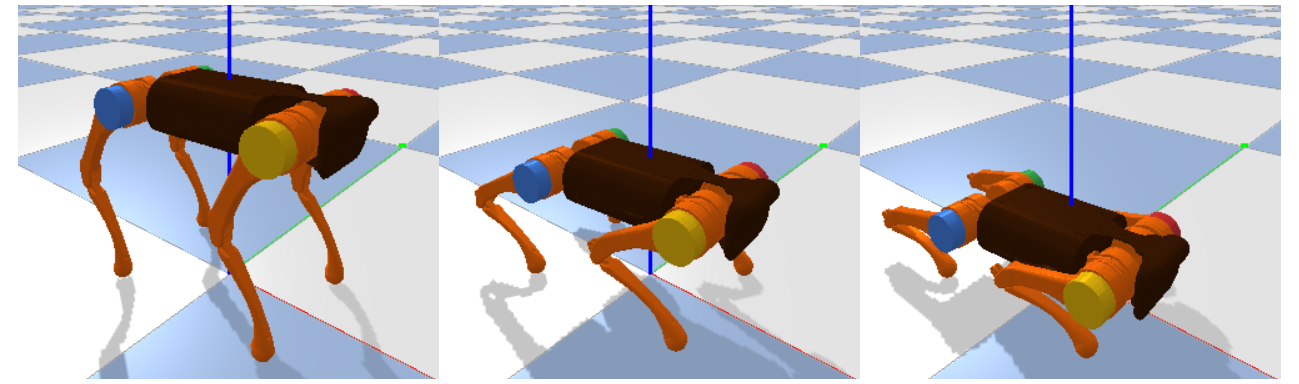
\includegraphics[width=0.8\textwidth]{figures/squatting.png}
    \caption{The result of squatting}
    \label{fig:squatting}
\end{figure}

In the initial position, the distance from hip joints to toe joints is 270. While the slider of debug parameter was pulled to the left, the distance became smaller, the body of robot descended vertically. While the slider of debug parameter was pulled to the right, the distance became larger, the body of robot ascended vertically.


\section{Error Analysis}

\subsection{Plane}

Without any operation after running the program, the robot would slide along the negative direction of the longitudinal axis. 




\subsection{}